Сервис был написан для:
\begin{itemize} 
\item проверки корректности работы платформы;
\item выявление возможных проблес, которые могут произойти на соревнованиях;
\item проведения тренировочной игры.
\end{itemize}

Сервис писался на языке Python с использованием микрофреймворка Flask.

Тестирование платформы заключалось в тестировании следующий функций:
\begin{itemize} 
\item Работа чекера (методы check, get, put);
\item Работа модуля сдачи флагов.
\end{itemize}

Смысл сервиса состоит в том, что в веб-приложении находится форма регистрации, которая сохраняет емайл и пароль в текстовый файл. На следующей странице есть форма, в которую нужно ввести емайл (введенный ранее в форму регистрации), после чего сервис выдает соответствующий пароль.

Несмотря на простоту сервиса, в нем содержится несколько уязвимостей:
\begin{itemize} 
\item секретный URL;
\item backdoor, с проверкой хеш-суммы емайла;
\item уязвимость path-traveling.
\end{itemize}

\begin{figure}[ht!]
\center{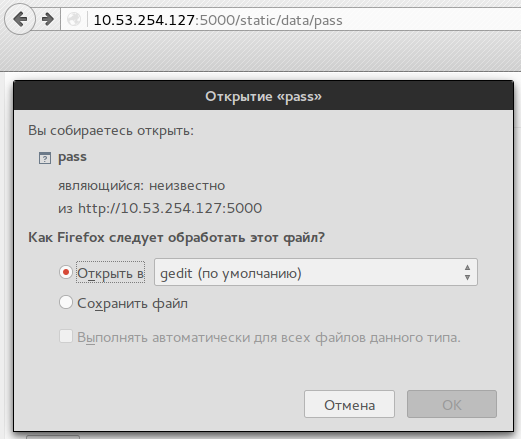
\includegraphics[width=0.8\linewidth]{eco/images/tima_u.png}}
\caption{Эксплуатирование уязвимости path-traveling}
\end{figure}